\documentclass{article}
\usepackage{tikz}
\usepackage{amssymb}
\usepackage{xcolor}

\usetikzlibrary{shapes,shapes.multipart}
\usetikzlibrary{arrows.meta}
\usetikzlibrary{positioning}
\begin{document}
\author{Nomair Yawar Bhatti}
\title{\textbf{Linked Lists Basics}}
\maketitle

\section{\color{red}{\textbf{Singly Linked List:}}}
\subsection{\color{blue}\textbf{Original Linked List:}}
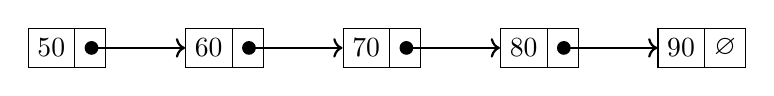
\begin{tikzpicture}
\tikzset{slinkedlist/.style={rectangle split, rectangle split horizontal,rectangle split parts=2,minimum width= 2cm,minimum height= 0.5cm}}
\node[slinkedlist,draw](a){$50$};
\node[slinkedlist,draw](b)[right=of a]{$60$};
\draw[thick,{Circle->}](a.two |- a.center) -- (b);
\node[slinkedlist, draw](c)[right=of b]{$70$};
\draw[thick,{Circle->}](b.two |- b.center) -- (c);
\node[slinkedlist,draw](d)[right=of c]{$80$};
\draw[thick,{Circle->}](c.two |- c.center) -- (d);
\node[slinkedlist,draw](e)[right=of d]{\nodepart{one}$90$\nodepart{two}$\varnothing$};
\draw[thick,{Circle->}](d.two |- d.center) -- (e);
\end{tikzpicture}
\newline\newline
This linked list consists of five nodes. Each node has an integer value and a pointer that points to the next node in the linked list.
The last node has a null pointer. It marks the end of the linked list.

\subsection{\color{blue}\textbf{Add node(65) to Linked List:}}
\begin{tikzpicture}
\newline
\tikzset{slinkedlist/.style={rectangle split, rectangle split horizontal,rectangle split parts=2,minimum width= 2cm,minimum height= 0.5cm}}
\node[slinkedlist,draw](a){$50$};
\node[slinkedlist,draw](b)[right=of a]{$60$};
\draw[thick,{Circle->}](a.two |- a.center) -- (b);
\node[slinkedlist, draw](c)[right=of b]{$70$};
\draw[draw=red,thick,{dashed}](b.two |- b.center) -- (c);
\node[slinkedlist,draw](d)[right=of c]{$80$};
\draw[draw,thick,{Circle->}](c.two |- c.center) -- (d);
\node[slinkedlist,draw](f)[right=of d]{\nodepart{one}$90$\nodepart{two}$\varnothing$};
\draw[thick,{Circle->}](d.two |- d.center) -- (e);
\node[slinkedlist, draw,fill=green](g)[above=of b ]{$65$};
\draw[draw=blue,thick,{Circle->}](b.two |- b.center) -- (g);
\draw[draw=blue,thick,{Circle->}](g.two |- g.center) -- (c);
\end{tikzpicture}
\newline\newline\newline
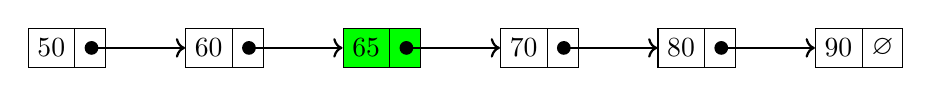
\begin{tikzpicture}
\tikzset{slinkedlist/.style={rectangle split, rectangle split horizontal,rectangle split parts=2,minimum width= 2cm,minimum height= 0.5cm}}
\node[slinkedlist,draw](a){$50$};
\node[slinkedlist,draw](b)[right=of a]{$60$};
\draw[thick,{Circle->}](a.two |- a.center) -- (b);
\node[slinkedlist, draw,fill=green](c)[right=of b]{$65$};
\draw[thick,{Circle->}](b.two |- b.center) -- (c);
\node[slinkedlist,draw](d)[right=of c]{$70$};
\draw[thick,{Circle->}](c.two |- c.center) -- (d);
\node[slinkedlist,draw](f)[right=of d]{$80$};
\node[slinkedlist,draw](e)[right=of f]{\nodepart{one}$90$\nodepart{two}$\varnothing$};
\draw[thick,{Circle->}](d.two |- d.center) -- (f);
\draw[thick,{Circle->}](f.two |- f.center) -- (e);
\end{tikzpicture}
\newline\newline 
A new node is added to the linked list. It has an integer value of \textcolor{orange}{\textbf{65}}. The node to be added is marked in green. The next pointer of 
the second node(\textcolor{orange}{\textbf{60}}) now points to the new node(\textcolor{orange}{\textbf{65}}). The next pointer of the new node(\textcolor{orange}{\textbf{65}}) points to the third node(\textcolor{orange}{\textbf{70}}) of the original linked list. The updated linked list has six nodes.

\subsection{\color{blue}\textbf{Delete node(80) from Linked List:}}
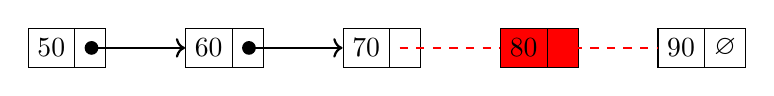
\begin{tikzpicture}
\tikzset{slinkedlist/.style={rectangle split, rectangle split horizontal,rectangle split parts=2,minimum width= 2cm,minimum height= 0.5cm}}
\node[slinkedlist,draw](a){$50$};
\node[slinkedlist,draw](b)[right=of a]{$60$};
\draw[thick,{Circle->}](a.two |- a.center) -- (b);
\node[slinkedlist, draw](c)[right=of b]{$70$};
\draw[thick,{Circle->}](b.two |- b.center) -- (c);
\node[slinkedlist,draw,fill=red](d)[right=of c]{$80$};
\draw[draw=red,thick,{dashed}](c.two |- c.center) -- (d);
\node[slinkedlist,draw](e)[right=of d]{\nodepart{one}$90$\nodepart{two}$\varnothing$};
\draw[draw=red,thick,{dashed}](d.two |- d.center) -- (e);
\end{tikzpicture}
\newline\newline\newline
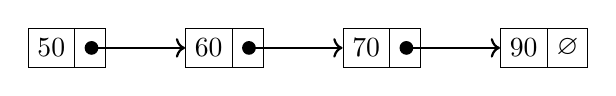
\begin{tikzpicture}
\tikzset{slinkedlist/.style={rectangle split, rectangle split horizontal,rectangle split parts=2,minimum width= 2cm,minimum height= 0.5cm}}
\node[slinkedlist,draw](a){$50$};
\node[slinkedlist,draw](b)[right=of a]{$60$};
\draw[thick,{Circle->}](a.two |- a.center) -- (b);
\node[slinkedlist, draw](c)[right=of b]{$70$};
\draw[thick,{Circle->}](b.two |- b.center) -- (c);
\node[slinkedlist,draw](d)[right=of c]{\nodepart{one}$90$\nodepart{two}$\varnothing$};
\draw[thick,{Circle->}](c.two |- c.center) -- (d);
\end{tikzpicture}
\newline\newline
An existing node(\textcolor{orange}{\textbf{80}}) is deleted from the linked list. The node to be deleted is marked in red. The next pointer of the third node(\textcolor{orange}{\textbf{70}}) points to the last node(\textcolor{orange}{\textbf{90}}).
The fourth node(\textcolor{orange}{\textbf{80}}) in the original linked list is removed. The updated linked list has four nodes.

\subsection{\color{blue}\textbf{Circular Linked List:}}
\begin{tikzpicture}
\useasboundingbox (-2,-0.15);
\tikzset{slinkedlist/.style={rectangle split, rectangle split horizontal,rectangle split parts=2,minimum width= 2cm,minimum height= 0.5cm}}
\node[slinkedlist,draw](a){$50$};
\node[slinkedlist,draw](b)[right=of a]{$60$};
\draw[thick,{Circle->}](a.two |- a.center) -- (b);
\node[slinkedlist, draw](c)[right=of b]{$70$};
\draw[thick,{Circle->}](b.two |- b.center) -- (c);
\node[slinkedlist,draw](d)[right=of c]{$80$};
\draw[thick,{Circle->}](c.two |- c.center) -- (d);
\node[slinkedlist,draw](e)[right=of d]{\nodepart{one}$90$};
\draw[thick,{Circle->}](d.two |- d.center) -- (e);
\draw[thick,{Circle-Stealth}](e.two |- e.center) to [out=-10,in=190,distance=5cm](a);
\end{tikzpicture}
\newline\newline\newline
In a singly circular linked list, the next pointer of the last node(\textcolor{orange}{\textbf{90}}) points to the first node(\textcolor{orange}{\textbf{50}}). 

\section{\color{red}\textbf{Doubly Linked List:}}
\subsection{\color{blue}\textbf{Original Linked List:}}
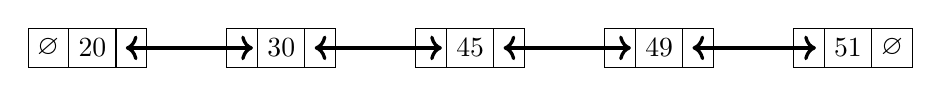
\begin{tikzpicture}
\tikzset{dlinkedlist/.style={rectangle split, rectangle split horizontal,rectangle split parts=3,minimum width= 2cm,minimum height= 0.5cm}}
\node[dlinkedlist,draw](a){\nodepart{one}$\varnothing$\nodepart{two}{$20$}};
\node[dlinkedlist,draw](b)[right=of a]{\nodepart{two}{$30$}};
\draw[very thick,{<->}](a.three |- a.center) -- (2.10,0);
\node[dlinkedlist, draw](c)[right=of b]{\nodepart{two}{$45$}};
\draw[very thick,{<->}](b.three |- b.center) -- (4.50,0);
\node[dlinkedlist,draw](d)[right=of c]{\nodepart{two}{$49$}};
\draw[very thick,{<->}](c.three |- c.center) -- (6.90,0);
\node[dlinkedlist,draw](e)[right=of d]{\nodepart{two}$51$\nodepart{three}$\varnothing$};
\draw[very thick,{<->}](d.three |- d.center) -- (9.25,0);
\end{tikzpicture}
\newline\newline
This linked list has five nodes. Each node has a previous pointer, an integer value and a next pointer. The previous pointer of the first node is Null.
The next pointer of the last node(\textcolor{orange}{\textbf{51}}) is null, and it marks the end of the doubly linked list.

\subsection{\color{blue}\textbf{Add node(47) to Linked List:}}
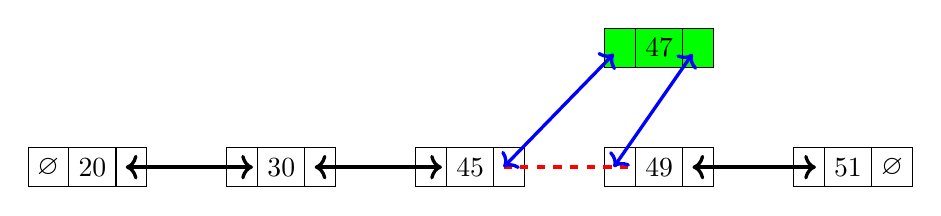
\begin{tikzpicture}
\tikzset{dlinkedlist/.style={rectangle split, rectangle split horizontal,rectangle split parts=3,minimum width= 2cm,minimum height= 0.5cm}}
\node[dlinkedlist,draw](a){\nodepart{one}$\varnothing$\nodepart{two}{$20$}};
\node[dlinkedlist,draw](b)[right=of a]{\nodepart{two}{$30$}};
\draw[very thick,{<->}](a.three |- a.center) -- (2.10,0);
\node[dlinkedlist, draw](c)[right=of b]{\nodepart{two}{$45$}};
\draw[very thick,{<->}](b.three |- b.center) -- (4.50,0);
\node[dlinkedlist,draw](d)[right=of c]{\nodepart{two}{$49$}};
\draw[draw=red,very thick,{dashed}](c.three |- c.center) -- (6.90,0);
\node[dlinkedlist,draw](e)[right=of d]{\nodepart{two}$51$\nodepart{three}$\varnothing$};
\draw[very thick,{<->}](d.three |- d.center) -- (9.25,0);
\node[dlinkedlist,draw,fill=green](f)[above=of d]{\nodepart{two}{$47$}};
\draw[draw=blue,very thick,{<->}](d.one |- d.center) -- (f.three);
\draw[draw=blue,very thick,{<->}](c.three |- c.center) -- (f.one);
\end{tikzpicture}
\newline\newline
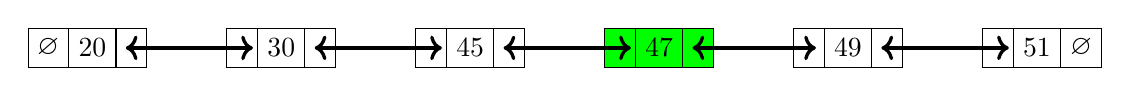
\begin{tikzpicture}
\tikzset{dlinkedlist/.style={rectangle split, rectangle split horizontal,rectangle split parts=3,minimum width= 2cm,minimum height= 0.5cm}}
\node[dlinkedlist,draw](a){\nodepart{one}$\varnothing$\nodepart{two}{$20$}};
\node[dlinkedlist,draw](b)[right=of a]{\nodepart{two}{$30$}};
\draw[very thick,{<->}](a.three |- a.center) -- (2.10,0);
\node[dlinkedlist, draw](c)[right=of b]{\nodepart{two}{$45$}};
\draw[very thick,{<->}](b.three |- b.center) -- (4.50,0);
\node[dlinkedlist,draw,fill=green](f)[right=of c]{\nodepart{two}$47$};
\draw[very thick,{<->}](c.three |- c.center) -- (6.90,0);
\node[dlinkedlist,draw](d)[right=of f]{\nodepart{two}{$49$}};
\draw[very thick,{<->}](f.three |- f.center) -- (9.25,0);
\draw[very thick,{<->}](d.three |- d.center) -- (11.70,0);
\node[dlinkedlist,draw](e)[right=of d]{\nodepart{two}$51$\nodepart{three}$\varnothing$};
\end{tikzpicture}
\newline\newline
A new node is added to the doubly linked list. The new node is marked in green. The previous pointer of the new node(\textcolor{orange}{\textbf{47}})
points to the third node (aka previous node,\textcolor{orange}{\textbf{45}}) of the original linked list. The next pointer of the new node(\textcolor{orange}{\textbf{47}}) points to the fourth node(\textcolor{orange}{\textbf{49}}) 
of the original linked list. Lastly, the previous pointer of the fourth node(\textcolor{orange}{\textbf{49}}) of the original linked list points to the new node(\textcolor{orange}{\textbf{47}}).

\subsection{\color{blue}\textbf{Delete node(45) from Linked List:}}
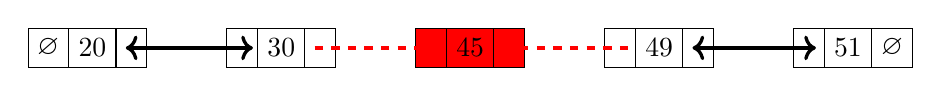
\begin{tikzpicture}
\tikzset{dlinkedlist/.style={rectangle split, rectangle split horizontal,rectangle split parts=3,minimum width= 2cm,minimum height= 0.5cm}}
\node[dlinkedlist,draw](a){\nodepart{one}$\varnothing$\nodepart{two}{$20$}};
\node[dlinkedlist,draw](b)[right=of a]{\nodepart{two}{$30$}};
\draw[very thick,{<->}](a.three |- a.center) -- (2.10,0);
\node[dlinkedlist, draw,fill=red](c)[right=of b]{\nodepart{two}{$45$}};
\draw[draw=red,very thick,{dashed}](b.three |- b.center) -- (4.50,0);
\node[dlinkedlist,draw](d)[right=of c]{\nodepart{two}{$49$}};
\draw[draw=red,very thick,{dashed}](c.three |- c.center) -- (6.90,0);
\node[dlinkedlist,draw](e)[right=of d]{\nodepart{two}$51$\nodepart{three}$\varnothing$};
\draw[very thick,{<->}](d.three |- d.center) -- (9.25,0);
\end{tikzpicture}
\newline\newline
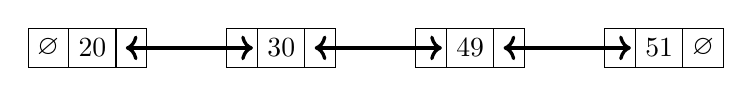
\begin{tikzpicture}
\tikzset{dlinkedlist/.style={rectangle split, rectangle split horizontal,rectangle split parts=3,minimum width= 2cm,minimum height= 0.5cm}}
\node[dlinkedlist,draw](a){\nodepart{one}$\varnothing$\nodepart{two}{$20$}};
\node[dlinkedlist,draw](b)[right=of a]{\nodepart{two}{$30$}};
\draw[very thick,{<->}](a.three |- a.center) -- (2.10,0);
\node[dlinkedlist,draw](d)[right=of b]{\nodepart{two}{$49$}};
\draw[draw,very thick,{<->}](b.three |- b.center) -- (4.50,0);
\node[dlinkedlist,draw](e)[right=of d]{\nodepart{two}$51$\nodepart{three}$\varnothing$};
\draw[very thick,{<->}](d.three |- d.center) -- (6.90,0);
\end{tikzpicture}
\newline\newline
An existing node(\textcolor{orange}{\textbf{45}}) is deleted from the linked list. The node to be deleted is marked in red.
The next pointer of the second node(\textcolor{orange}{\textbf{30}}) points to the fourth node(\textcolor{orange}{\textbf{49}}) of the original linked list. The previous pointer of the
fourth node(\textcolor{orange}{\textbf{49}}) points to the second node(\textcolor{orange}{\textbf{30}}) of the linked list (refer to 2.1). The updated linked list has four nodes.
\end{document}


